\chapter{Literature Review}
\label{cap:cap02}

OpenFlow is the central theme of this project and the OpenFlow 1.3 specification \cite{ofspec13} is the main document of our bibliographic base. For this reason, a deep study of the protocol and technologies that use it was carried out. We have evaluated and compared available implementations of other OpenFlow software switches. Also, some tools required evaluate our work are worth mentioning. We investigated controllers, test frameworks and packet dissectors, all candidates to compose our OpenFlow test environment. The next sections will give an overview about OpenFlow and relevant tools related to this work. 

\section{OpenFlow}
\label{sec:sec21}

OpenFlow is an open standard communication interface between switches and controllers, allowing centralized control and programmability in the network. The basic OpenFlow switch is composed by one or more flow tables, a group table and one or more OpenFlow channels for communication with OpenFlow controllers. Figure \ref{fig:logicalswitch} is a logical view of the minimal elements required by an OpenFlow switch. 

\begin{figure}[H]
\centering
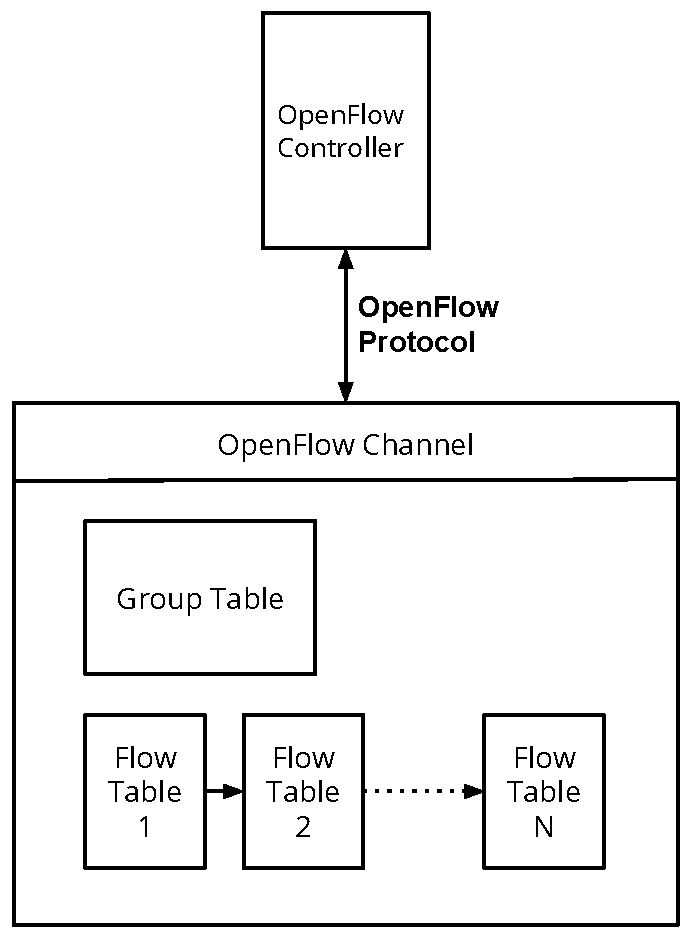
\includegraphics[height=8cm,width=\textwidth,keepaspectratio]{cap2/OFSwitch.pdf}
\caption{OpenFlow switch minimal elements.}
\label{fig:logicalswitch}
\end{figure}
\pagebreak

OpenFlow controllers can install flows into the switch flow table. A flow consists of match fields, counters and instructions applied to matching packets. A packet matches a flow if the protocol header field's values are the same as those specified in flow match fields. The most recent version requires 13 match fields, shown by Table \ref{tab:OFRequired}, but has optional support for more than 30 protocols fields from layers 2, 3 and 4 of TCP/IP network stack.

The OpenFlow pipeline starts at the first flow table and continues to additional tables. Flows are matched in order of priority and the associated instructions are executed. Only two instructions are required for OpenFlow switches: \textit{Write-Actions}, in which actions are executed at the end of the pipeline, and \textit{Goto-Table}, to jump to tables with an id greater than the table where the instruction is executed. Optional instructions are \textit{Meter}, to direct the packet to some meter for Quality of Service (QoS), \textit{Apply-Actions}, for immediate action application, \textit{Clear-Actions}, to clear all actions written by a \textit{Write-Actions} instruction, and \textit{Write-Metadata}, to write metadata information to be carried across the tables. 

\begin{table}[H]
\caption{OpenFlow required match fields}\label{tab:OFRequired}
\centering
\begin{tabular}{|l|l|}
\hline
\textbf{Field} & \textbf{Description}                \\ \hline
Inport         & Ingress Port                        \\ \hline
Eth Dst        & Ethernet destination address         \\ \hline
Eth Src        & Ethernet source address              \\ \hline
Eth Type       & Type of the packet, after VLAN tags \\ \hline
IP Proto       & IPv4 or IPv6 next protocol number   \\ \hline
IPv4 Src       & IPv4 source address                 \\ \hline
IPv4 Dst       & IPv4 destination address             \\ \hline
IPv6 Src       & IPv6 source address                 \\ \hline
IPv6 Dst       & IPv6 destination address            \\ \hline
TCP Src        & TCP source port                     \\ \hline
TCP Dst        & TCP destination port                \\ \hline
UDP Src        & UDP source port                     \\ \hline
UDP Dst        & UDP destination port                \\ \hline
\end{tabular}
\label{my-label}
\end{table}

Actions can perform modifications on packets, discard or send them to the group table or simply output to some specific port. The only required actions are \textit{Output}, to send the packet through a port, and \textit{Drop}. The packet modification actions are all optional, but their implementation is recommended, as they give more power and options to OpenFlow networks. The optional actions are \textit{Group}, to process the packet through a specific group; \textit{Push-Tag/Pop Tag}, for addition and deletion of VLAN, MPLS and PBB tags; \textit{Set-Field}, to modify packets header fields; \textit{Change TTL}, an action to modify MPLS and IP TLL; \textit{Set-Queue}, to determine which queue is attached to a port and will be used for scheduling in packet forwarding.

OpenFlow groups are a way to perform more complex forwarding actions. When a packet is sent to a group it is cloned and executed by sets of action buckets. This abstraction enables flooding, multipath, link aggregation and other techniques that demand transmission of packets through more than one port. 

The last essential block is the OpenFlow channel. The main connection between controller and switch is done by one of the following transport protocols: TCP or TLS, where the second is recommended because it enables data encryption of the transmitted data. Auxiliary connections are also allowed and it is possible to have UDP connections for transmission of less sensitive OpenFlow messages.

An optional element of the OpenFlow switch is the Meter Table. This table comprises different types of Meter Bands, which have a speed limit and apply a determined QoS action in the case of a packet flow exceeding the determined limit. There are two types of bands covered by the OpenFlow 1.3 specification: \textit{Drop}, to discard packets; and \textit{DSCP Remark}, to decrease the drop precedence of the DSCP field of the IP header.

\subsection{One day in the life of an OpenFlow 1.3 switch in 10 steps}

To illustrate the operation of an OpenFlow switch we will present a common and simple example for new SDN learners. A learning switch is a layer 2 network equipment that learns the port to which a host is connected. Learning happens when a packet from a host arrives at the switch for the first time. The switch then obtains and stores the host Media Access Control (MAC) address associated with the port number. Next time, when another host sends a packet to the previous learned address, the switch will forward it directly, instead of flooding to all ports. 

In legacy devices, the control software is embedded into the switch hardware and the MAC addresses are stored in a Content Addressable Memory (CAM) table. In an OpenFlow scenario, the learning happens inside the controller and the forwarding rules are stored in the Flow Table. We will describe the steps of learning and forwarding processes of an OpenFlow switch controlled by a simple learning switch application, considering the topology in Figure \ref{fig:simpletopo}. 

\begin{figure}[H]
\centering
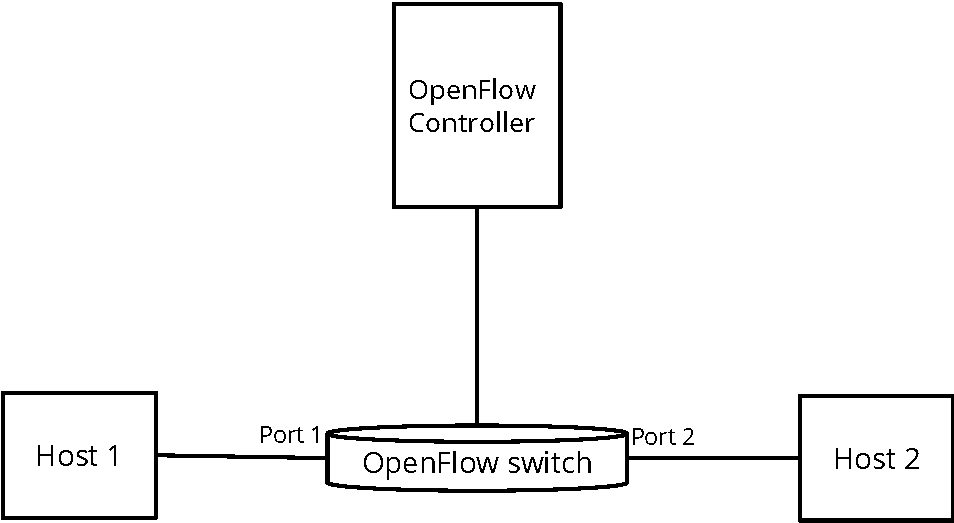
\includegraphics[height=5cm,width=\textwidth,keepaspectratio]{cap2/SimpleTopology.pdf}
\caption{Simple topology for the learning switch example.}
\label{fig:simpletopo}
\end{figure}

In the initial state the switch Flow Table is empty, \textit{Host 1} and \textit{Host 2} do not know anything about each other and the  \textit{Controller} is about to connect with the \textit{Switch}. 

\begin{enumerate}

\item The \textit{Controller} establishes a connection with the \textit{Switch}. As packets sent to an empty Flow Table are dropped according to the OpenFlow 1.3 specification, the  \textit{Controller} installs a low priority flow to direct every non matching packet to him. Table \ref{tab:initialtable} shows the Flow Table state after the installation of the first flow.  

\begin{table}[H]
\centering
\caption{Switch Flow Table state after controller connection}
\label{tab:initialtable}
\begin{tabular}{|l|l|l|}
\hline
\textbf{Match}  & \textbf{Priority} & \textbf{Instruction}                              \\ \hline
all             & 0                 & apply actions -> output:controller                \\ \hline
\end{tabular}
\end{table}

\item \textit{Host 1} wants to transmit a file to \textit{Host 2}. As it does not know about \textit{Host 2} MAC address, it sends an ARP \cite{rfc826} request to the network.

\item The ARP request packet enters the \textit{Switch} and matches the unique flow installed in the Flow Table. The action is applied, sending the packet to the  \textit{Controller} in an OpenFlow \textit{Packet In} message.

\item The  \textit{Controller} receives the \textit{Packet In}. The message contains information about the packet input port and headers. The  \textit{Controller} application learns and stores the \textit{Host 1} input port and MAC address. After that, it sends a \textit{Packet Out} message back to the \textit{Switch}, with an action to flood the packet in every \textit{Switch} port.   

\item The \textit{Packet Out} message arrives at the \textit{Switch} and the packet is flooded to every port, except the port where it came from.

\item The ARP request is delivered to \textit{Host 2}. Then, an ARP reply is sent back with the \textit{Host 2} MAC address required by \textit{Host 1}.

\item The ARP reply arrives at the \textit{Switch}. It matches the only present flow and is sent in a \textit{Packet In} message to the  \textit{Controller}.   

\item Now, the  \textit{Controller} checks if the packet MAC address is known. As the address is not present, it stores the input port and the MAC. Now it checks if the destination address was stored previously. The destination to \textit{Host 1} is already known. The  \textit{Controller} installs a new flow into the \textit{Switch} Flow Table. The flow illustrated in the second row of Table \ref{tab:secondtable} matches every packet destined to \textit{Host 1} MAC address and outputs the packet into port 1. After installing the flow, it sends the ARP reply to the \textit{Switch}, encapsulated in a \textit{Packet Out} message.

\begin{table}[H]
\centering
\caption{Switch Flow Table state after learning Host 1 address}
\label{tab:secondtable}
\begin{tabular}{|l|l|l|}
\hline
\textbf{Match}                 & \textbf{Priority}   & \textbf{Instruction}                              \\ \hline
all                            & 0                   & apply actions -> output:controller                \\ \hline
eth dst:HOST 1 MAC             & 100                 & apply actions -> output:1                         \\ \hline
\end{tabular}
\end{table}

\item This time The ARP reply is not flooded to all ports. As the  \textit{Controller} knew about the destination, it is sent directly to \textit{Host 1}. After receiving the ARP reply, it starts transmitting the file to \textit{Host 2}.

\item Again, the first packet of the file transference to \textit{Host 2} is sent to the  \textit{Controller}. Now it knows about \textit{Host 2} MAC and origin port. It installs another flow, shown in the third row of Table \ref{tab:finaltable}, and it sends the \textit{Packet Out} message to the \textit{Switch}. The \textit{Switch} sends the packet directly to \textit{Host 2}. From now on, the packets are not sent for the \textit{Controller} anymore because the installed flows are matched. 

\begin{table}[H]
\centering
\caption{Switch Flow Table final state}
\label{tab:finaltable}
\begin{tabular}{|l|l|l|}
\hline
\textbf{Match}                 & \textbf{Priority}   & \textbf{Instruction}                              \\ \hline
all                            & 0                   & apply actions -> output:controller                \\ \hline
eth dst:HOST 1 MAC             & 100                 & apply actions -> output:1                         \\ \hline
eth dst:HOST 2 MAC             & 100                 & apply actions -> output:2                         \\ \hline
\end{tabular}
\end{table}


\end{enumerate}        

\section{OpenFlow software switches}
\label{sec:sec22}

OpenFlow software switches play an important role in the protocol evolution. At first, they were a low cost solution to create and experiment your own SDN applications in a controlled and smaller environment, before the deployment in a production environment. With the new SDN approaches for network virtualization \cite{Tseng:2011:NVC:2117686.2118540} \cite{Drutskoy_scalablenetwork}, software switches have been receiving a lot of attention from the industry \cite{NSX} and academy \cite{DBLP:confcloudnetEmmerichRWC14}. SDN virtual switches interconnect virtual machines from data center tenants and help scaling a plethora of traffic engineering applications. For instance, tenant isolation is easily achieved using an OpenFlow software switch to connect virtual machines. Usually, it is implemented using VLAN segregation, which is not scalable for more than 4096 tenants (the total number of possible VLAN identifiers). In turn, OpenFlow switches offer more granular options to segregate the network hosts, due to the number of fields available for flow matching, which eliminates the need to segregate hosts only in a layer 2 domain.

\begin{table}[H]
\caption{Comparison of OpenFlow software switches}
\label{tab:relatedswitches}
\begin{tabular}{|l|l|l|l|l|}
\hline
\textbf{Switch} & \textbf{Language} & \textbf{Emulation tool integration} & \textbf{Mode}    & \textbf{OF-Config} \\ \hline
Reference       & C                 & Yes                        & userspace        & No                         \\ \hline
Open vSwitch    & C                 & Yes                        & userspace/kernel & No                         \\ \hline
LINC            & Erlang            & No                    & userspace        & Yes                        \\ \hline
Trema           & C/Ruby            & No                    & userspace        & No                         \\ \hline
\end{tabular}
\end{table}

Before the implementation, we investigated four OpenFlow software switches that supported OpenFlow 1.0, since there was no sense in implementing basic OpenFlow features from scratch. Table \ref{tab:relatedswitches} is a comparison of the examined software switches and reflects their state in the year of 2012. The columns are related to the objectives defined in chapter \ref{cap:intro}. Language is an important element, since popular programming languages have the power to reach bigger audiences. The integration with emulation tools eases experimentation and speeds up testing. The mode column is related to switch performance, since a kernel space implementation tend to be more efficient than an user space implementation. In a kernel implementation, packets are processed directly in the kernel space, eliminating the overhead of traversing packets between the kernel and user space.

In the mean time of this work, most of the analysed software switch projects started to add support for newer OpenFlow versions. Figure \ref{fig:ofswitchtimeline} shows the switche's timeline for the implementation of most recent OpenFlow versions. Colored intervals show that these OpenFlow versions are still in progress or do not include all features described on the specification, as will be shown in section \ref{sec:FeatureComplete}.

\begin{figure}[H]
\centering
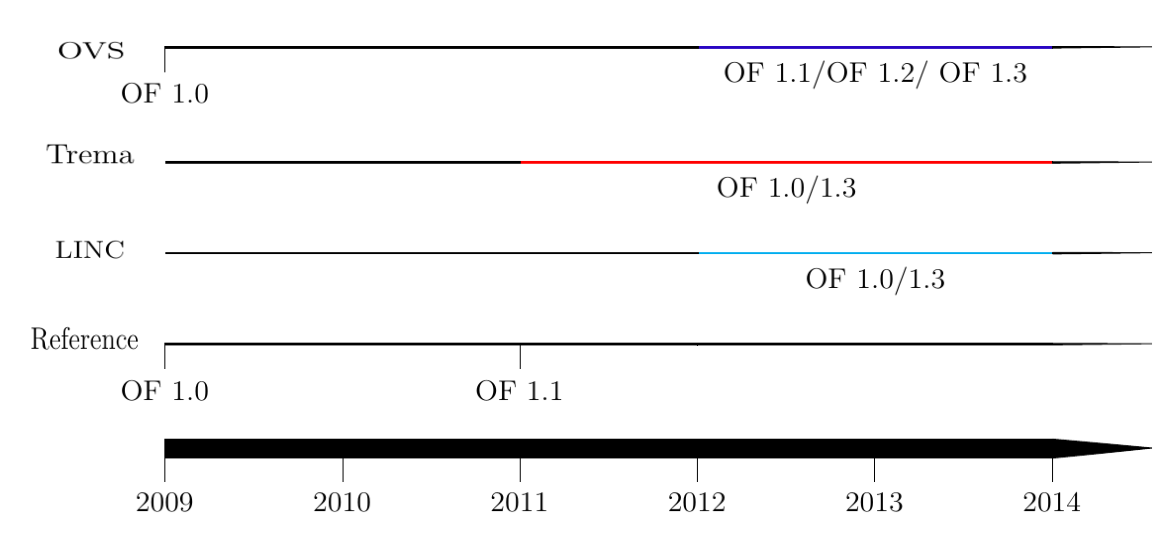
\includegraphics[height=6cm,width=\textwidth,keepaspectratio]{cap2/SoftSwitchTimeline.pdf}
\caption{OpenFlow Software Switches: version support timeline.}
\label{fig:ofswitchtimeline}
\end{figure}

The next subsections will provide a short individual description of the software switches investigated: OpenFlow reference switch, Open vSwitch, LINC and Trema. 

    \subsection{OpenFlow reference switch}
    \label{sec:sec221}
    
     The first OpenFlow switch is known as reference switch because it was implemented by Stanford researchers directly involved with the OpenFlow protocol creation and the first specification releases. The code is written using the C language and its simplicity is one of the reasons for the implementation to other platforms. Two important ports are: NetFPGA boards \cite{netpfgaof}, eliminating the disadvantage of the user space implementation; and OpenWrt \cite{pantou} for wireless routers. These efforts enabled low cost options to test OpenFlow on real hardware during earlier protocol stages.    
     
     The last OpenFlow version implemented by Stanford researchers was 1.0, but after the version 1.1 release there was an update, based on the reference switch, released by Ericsson Traffic Lab, called of11softswitch \cite{of11softswitch}. To conform changes such as multiple tables, the switch forwarding plane was rewritten, but still retained all of the base software switch characteristics.     

     \subsection{Open vSwitch}
    
    Considered the \texttt{de facto} switch for virtual networks, Open vSwitch \cite{Pfaff_e.a.:extending} (OVS) is a mature and constantly evolving open source project. The efficiency provided by the kernel module and the functionalities beyond OpenFlow turns OVS into a great solution to replace the original Linux bridge. Although high performance is guaranteed by the kernel module, it makes the OVS code harder to insert new functionalities. 
    
    In addition to the basic connectivity provided by traditional bridges, OVS offers a flexible option to manage and program the packet forwarding behavior. OVS uses another protocol than OpenFlow for switch management. The Open vSwitch Database Management Protocol (OVSDB) is one of the most praised OVS features and is designed to manage all running switch instances, permitting the control of distributed virtual network nodes. With OVSDB, a network engineer can create, configure and delete OVS ports and tunnels from a centralized location.

    \subsection{LINC}
    
    LINC \cite{linc} is an userspace software switch written in the Erlang programming language and has different support levels, considering the number of working features, for OpenFlow versions from 1.2 to 1.4. The main advantage of this switch is the support to OF-CONFIG \cite{ofconfig}, the OpenFlow switch configuration protocol. As an userspace implementation, efficiency is not one of its strong points. However, it promises flexibility, fast development and testing of new OpenFlow features. 
    The Erlang language is not a disadvantage \textit{per se}, but it can be considered a blocking point for developers who want to add their own features. Erlang developers are growing, but their number are still very far from languages like C and Java.

    \subsection{Trema}
    
    Trema is a name known by the OpenFlow community for being a controller implementation project. However it goes beyond,  offering a full OpenFlow framework with the tools needed to develop OpenFlow applications \cite{trema}, including an OpenFlow software switch. Also, the framework has its own emulation tool for OpenFlow networks and end-hosts. The main repository of this project features switch with only OpenFlow 1.0. However, there is a repository known as trema-edge where the work for OpenFlow 1.3 is on progress.

\section{OpenFlow Controllers}

    Controllers are considered the brain of an OpenFlow network. Every configuration and forwarding rules are defined by applications running on top of a controller. They are sent in form of OpenFlow messages, which have to conform with the format defined by the specification. For this reason, we need to validate our work testing interoperability between the software switch and a compliant controller. We reviewed the main open source projects, looking for an OpenFlow 1.3 controller or an easy alternative to implement some level of support for OpenFlow 1.3, required for our tests. 

    \subsection{NOX}

    One of the first open source OpenFlow controllers, NOX \cite{nox} was very famous during the first years of OpenFlow. Its popularity was due to a combination of factors, from the C++ implementation and a Python binding, which helped to speed up the prototyping, to a quite simple interface and a good number of example applications. The last official release supported OpenFlow 1.0 version. After some enhancements on the controller speed \cite{nox-mt}, no efforts were made to upgrade it for newer OpenFlow versions. 
    
    \subsection{POX}
    
    Pox is a controller implemented in Python and can be considered a NOX sibling \cite{pox}, created to address the lack of speed when prototyping with NOX. Its main goal is to become the archetypal of a modern SDN controller, featuring some desired SDN capabilities like debugging, new programming models and network virtualization. 
    
    Designed with research in mind, under constant development and a typical controller used for SDN education, POX was a great candidate to be the controller for testing the software switch, but the OpenFlow support still doesn't surpass version 1.0
  
    \subsection{Floodlight}

    The Floodlight controller is a popular OpenFlow controller backed by Big Switch Networks, one of the most prominent SDN startups \cite{floodlight}. It is developed in Java and was designed for high performance and is the core of Big Switch Networks' commercial solution. One of the greatest features of Floodlight is the module loading system that makes it very extensible, allowing it to enable and disable applications at run time. Another great feature is the Open Stack integration, a cloud orchestration platform. Floodlight instances control the virtual switches linking virtual machines orchestrated by Open Stack. Regarding OpenFlow version support, it currently supports OpenFlow 1.0 and 1.3. 
  
    \subsection{Ryu}
    
    Ryu is considered an SDN network framework \cite{ryu}, an abstraction that provides code software components, with generic functionality, easing and speeding development of SDN applications. It is implemented in Python, like POX, but has a different architecture. Designed as software components, developers can create OpenFlow applications like modules. Furthermore, the controller also supports management protocols like OF-Config and Netconf.
    
    Very well documented, with a large number of examples and featuring all OpenFlow versions, Ryu is currently a great choice to test the software switch, but when we started this work OpenFlow support was limited to OpenFlow 1.0. OpenFlow 1.3 support was only available in the middle of our switch implementation.
 

\section{OpenFlow test and emulation}
\label{sec:testemulation}
    The last pieces of a minimal OpenFlow environment are  test frameworks and emulation tools. For our development we are more interested in the first, though a modular emulation software compatible with our software switch may benefit users looking for a complete, controlled and easy to setup testbed. 
    
    \subsection{OF-Test}
    
    OF-Test was the first OpenFlow test framework. Developed by the same team working on Floodlight, OF-Test \cite{oftest} tests basic functionality for OpenFlow 1.0 and 1.1, with 1.2 and 1.3 currently in development. The simpler architecture and Python implementation turns it into a very easy and fast platform to create and run tests. It works connecting the OF-test server to the switch control and the data plane. The server is responsible for monitoring OpenFlow messages and packets sent through and along the planes. If these messages and packets are according to expected results, the test returns OK, otherwise, a failure is reported.
    
    \subsection{Ryu Test Framework}
    
    This test framework is part of the Ryu controller and implements tests to cover all, required and optional, OpenFlow 1.3 and 1.4, actions, instructions and match fields, with a more comprehensive test than OF-Test. The test cases are written in JSON, so there is no need for coding to create a test, which enhances the speed of test creation. 
    
    There is an online certification which continuously tests OpenFlow software and hardware switches, including our work \cite{ryucert}. Results from this certification will be presented in chapter \ref{cap:cap05}.

    \subsection{OpenFlow packet dissectors}

    Packet dissectors are important tools to test if message packets are correct or to check if an specific packet was sent or modified by an OpenFlow output and set-field actions, respectively. Wireshark \cite{wireof} is the most famous program to dissect packets. Although a wide range of protocols are officially supported, OpenFlow support started as an  unofficial  plugin for OpenFlow 1.0 and 1.1. For a long time this plugin was the only option for analyzing OpenFlow traffic. Recently, due to the growth in the number of users requesting for official support, OpenFlow is now developed in the dissector's main repository \cite{wireof}.    
    \subsection{Mininet}
    
   Mininet \cite{Lantz:2010:NLR:1868447.1868466} is a tool for network emulation. In a single machine it runs switches, links and hosts just like a complete virtual network. It is possible to log into the hosts and use programs like Iperf \cite{iperf} and Ping, to measure throughput and check connectivity; specify link parameters as speed and delay; and instantiate a network topology composed of software switches. The capacity to create and to destroy virtual networks allows fast and easy experimentation. 
  
    